
\subsection{Results}

\subsubsection{Evaluation for Counting Queries}

\begin{figure*}[t]
  \centering
  
\includegraphics[width=.4\linewidth]{figs/legend_methods.pdf}

  \subfloat[Cosmetics ($w=20$)]{%
    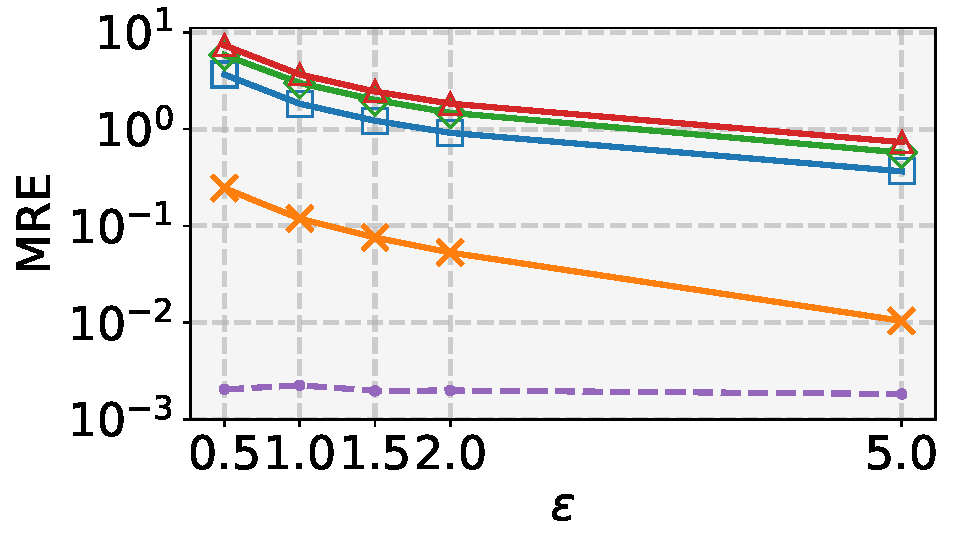
\includegraphics[width=.25\linewidth]{figs/w=20-category.pdf}}
  \subfloat[Cosmetics ($\epsilon=1$)]{%
    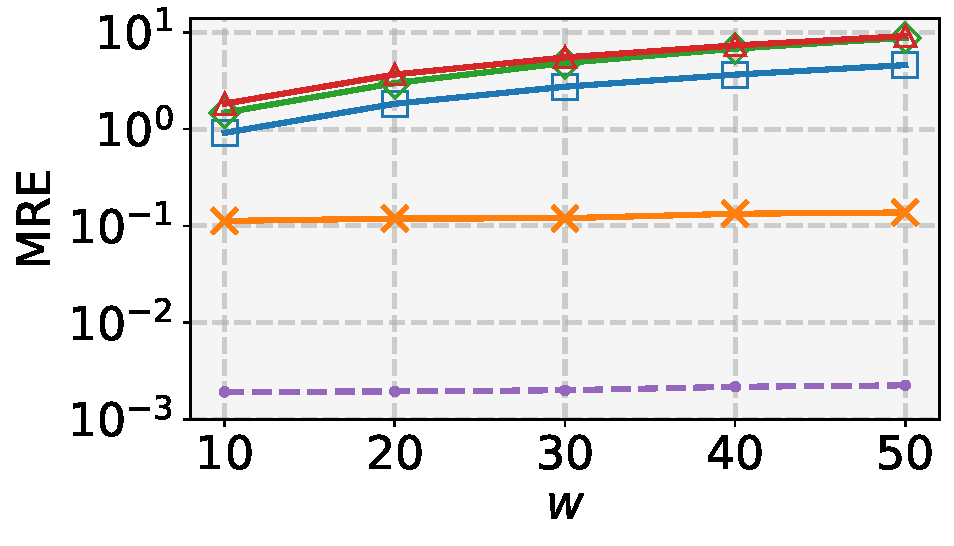
\includegraphics[width=.25\linewidth]{figs/e=1-category.pdf}}
  \subfloat[Cosmetics ($w=20$)]{%
    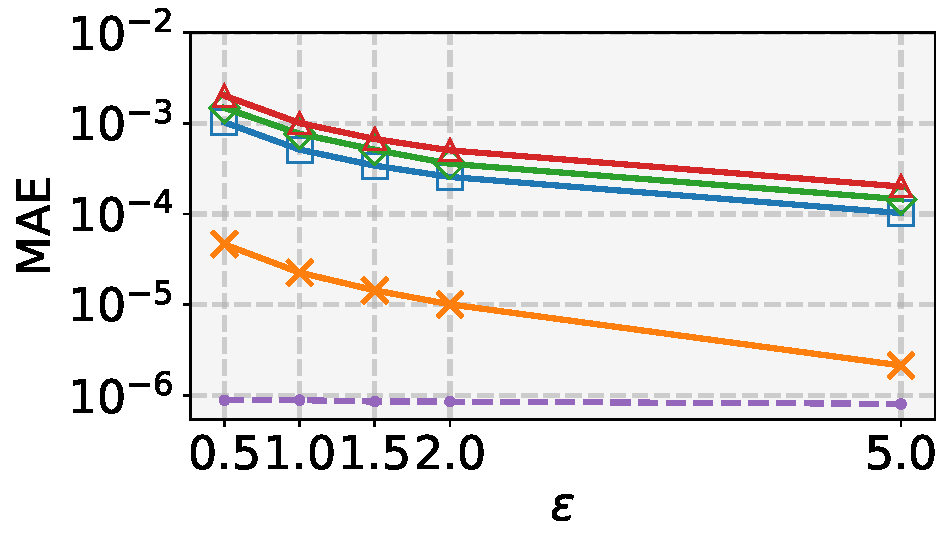
\includegraphics[width=.25\linewidth]{figs/w=20-category-MAE.pdf}}
  \subfloat[Cosmetics ($\epsilon=1$)]{%
    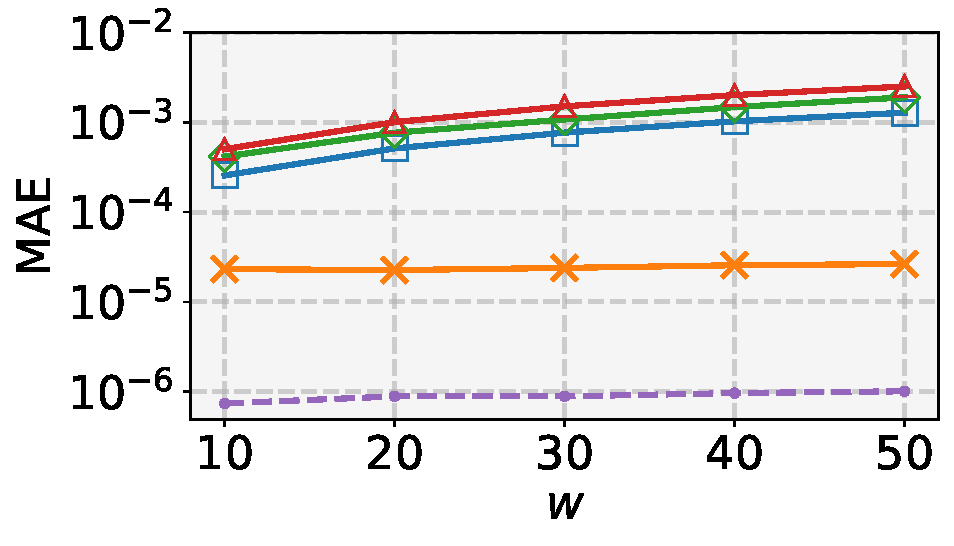
\includegraphics[width=.25\linewidth]{figs/e=1-category-MAE.pdf}}

  \subfloat[Taxi ($w=20$)]{%
    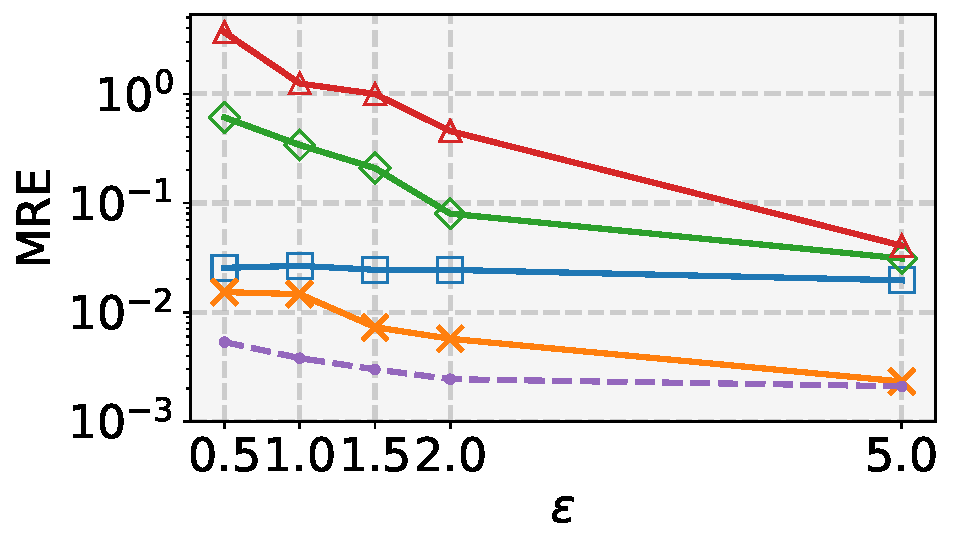
\includegraphics[width=.25\linewidth]{figs/w=20-taxi.pdf}}
  \subfloat[Taxi ($\epsilon=1$)]{%
    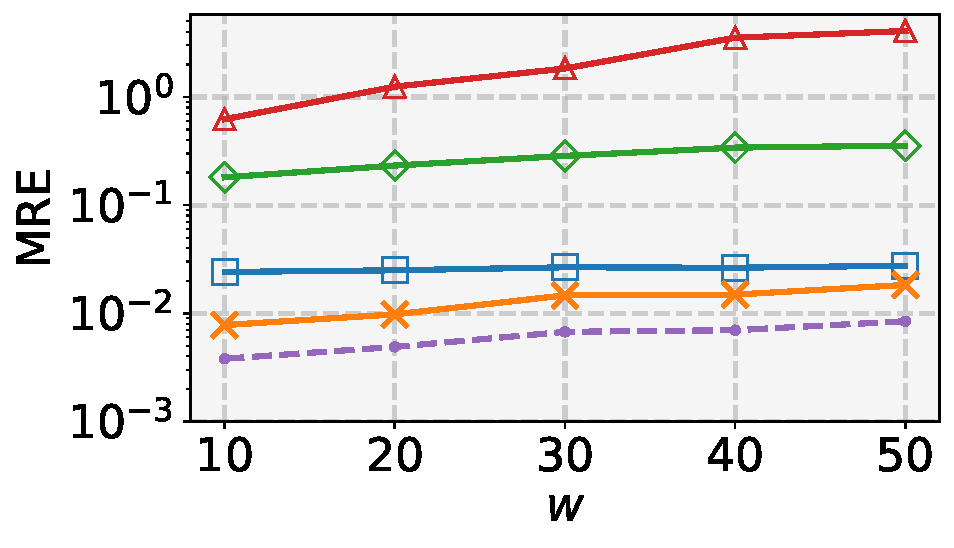
\includegraphics[width=.25\linewidth]{figs/e=1-taxi.pdf}}
  \subfloat[Taxi ($w=20$)]{%
    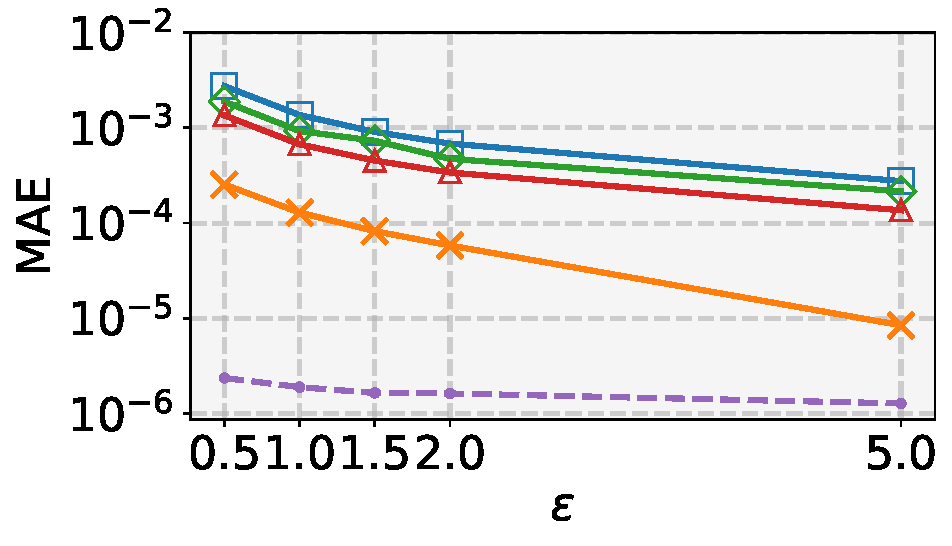
\includegraphics[width=.25\linewidth]{figs/w=20-taxi-MAE.pdf}}
  \subfloat[Taxi ($\epsilon=1$)]{%
    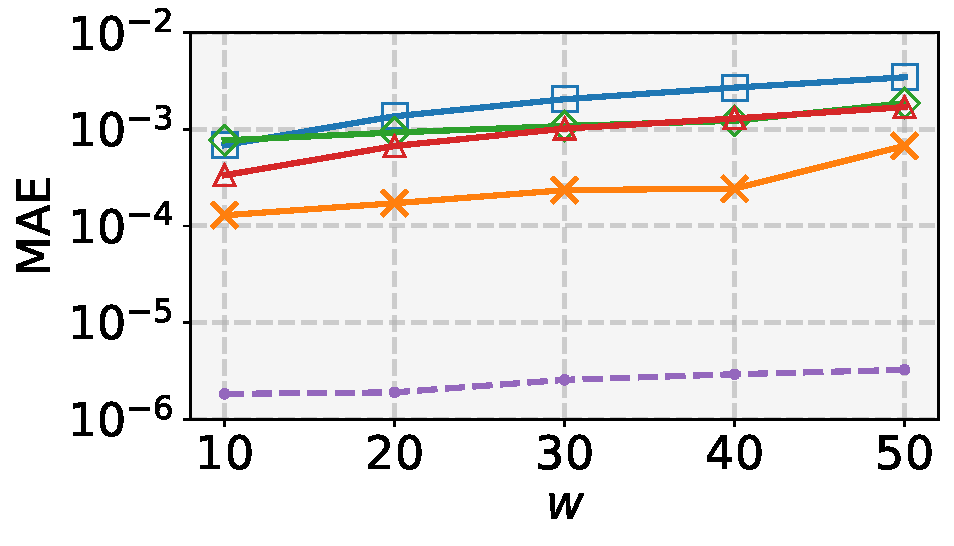
\includegraphics[width=.25\linewidth]{figs/e=1-taxi-MAE.pdf}}

  \subfloat[Loan ($w=20$)]{%
    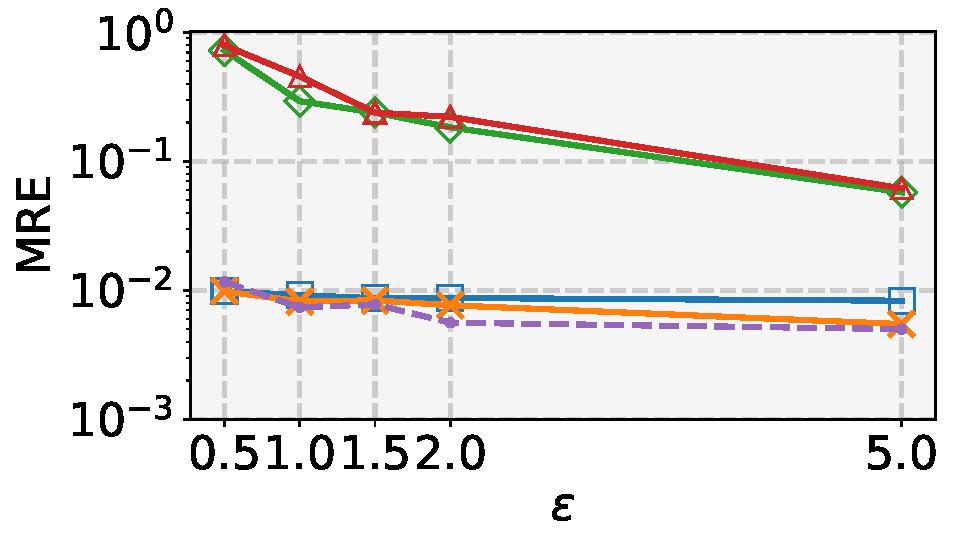
\includegraphics[width=.25\linewidth]{figs/w=20-loan.pdf}}
  \subfloat[Loan ($\epsilon=1$)]{%
    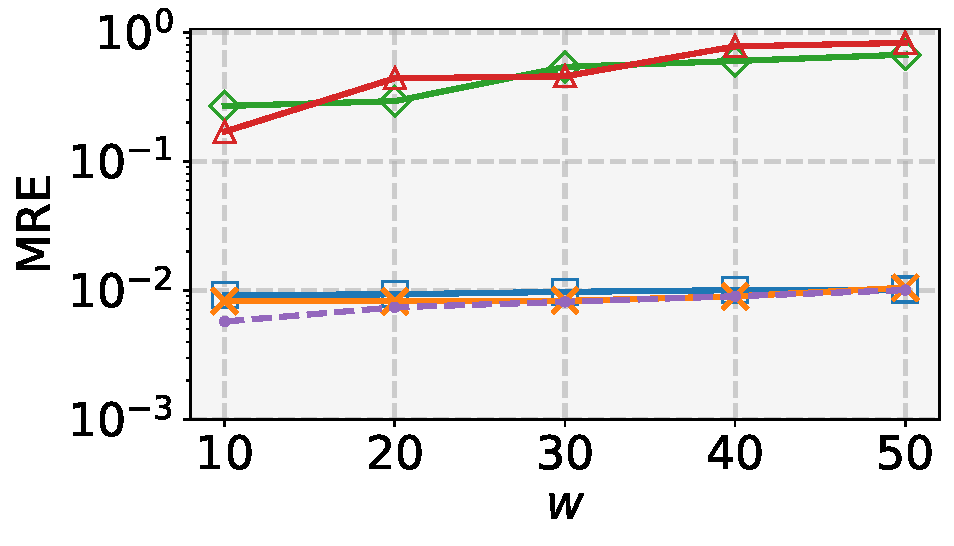
\includegraphics[width=.25\linewidth]{figs/e=1-loan.pdf}}
  \subfloat[Loan ($w=20$)]{%
    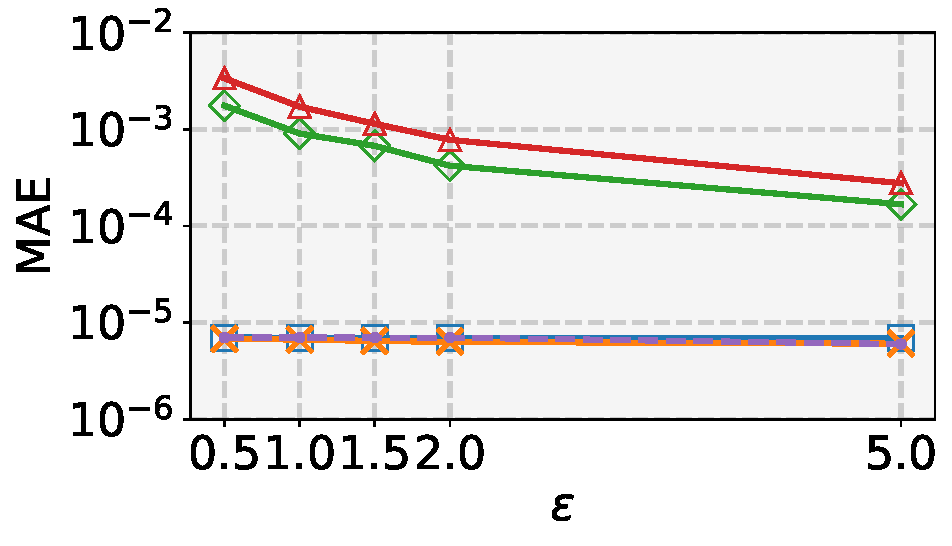
\includegraphics[width=.25\linewidth]{figs/w=20-loan-MAE.pdf}}
  \subfloat[Loan ($\epsilon=1$)]{%
    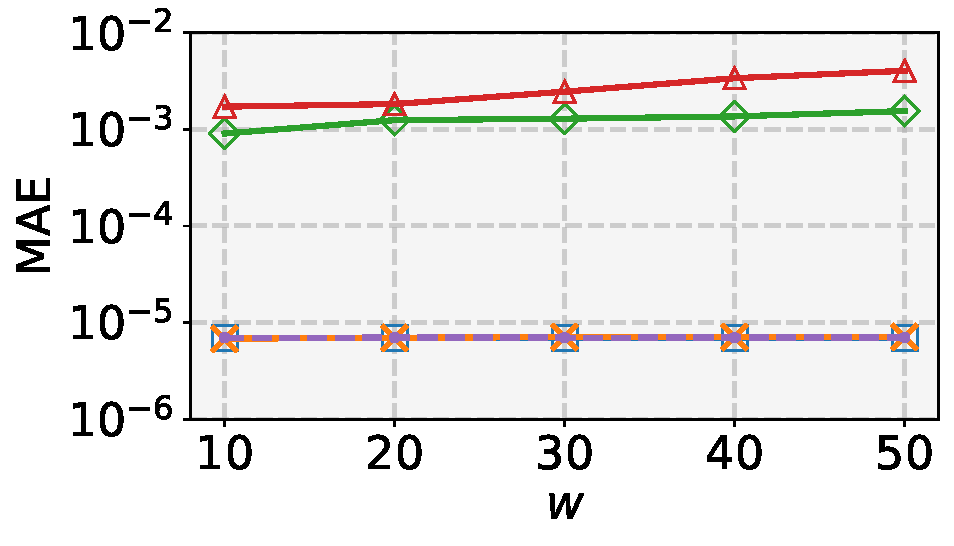
\includegraphics[width=.25\linewidth]{figs/e=1-loan-MAE.pdf}}

  \subfloat[Foursquare ($w=20$)]{%
    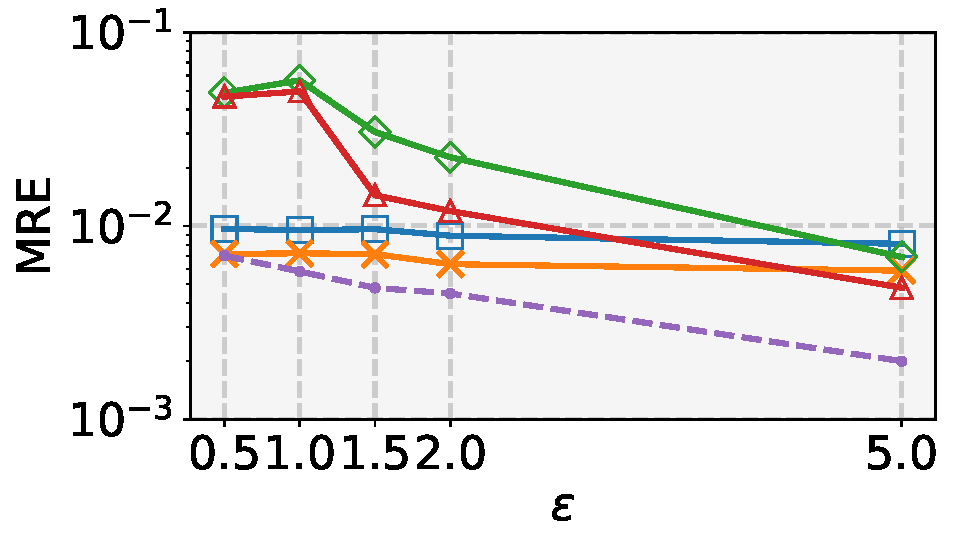
\includegraphics[width=.25\linewidth]{figs/w=20-tist.pdf}}
  \subfloat[Foursquare ($\epsilon=1$)]{%
    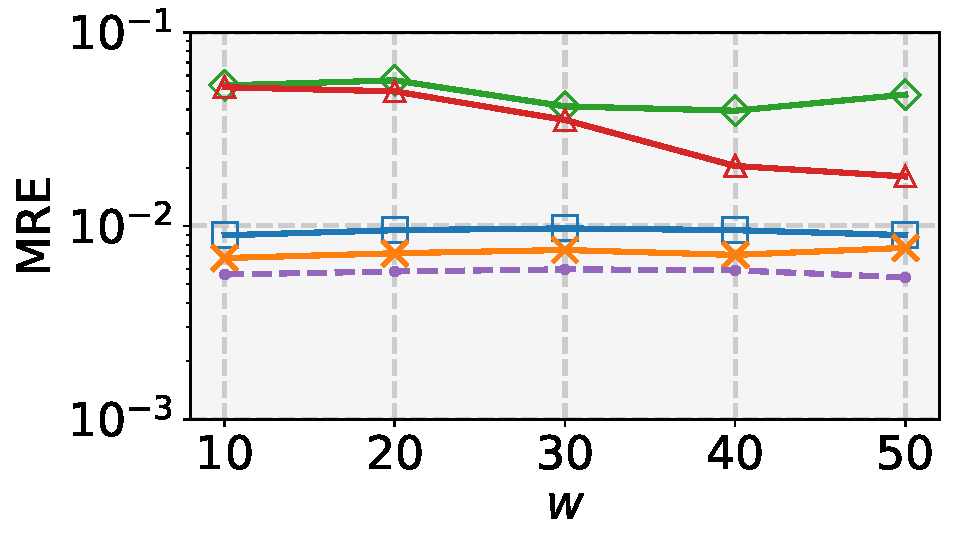
\includegraphics[width=.25\linewidth]{figs/e=1-tist.pdf}}
  \subfloat[Foursquare ($w=20$)]{%
    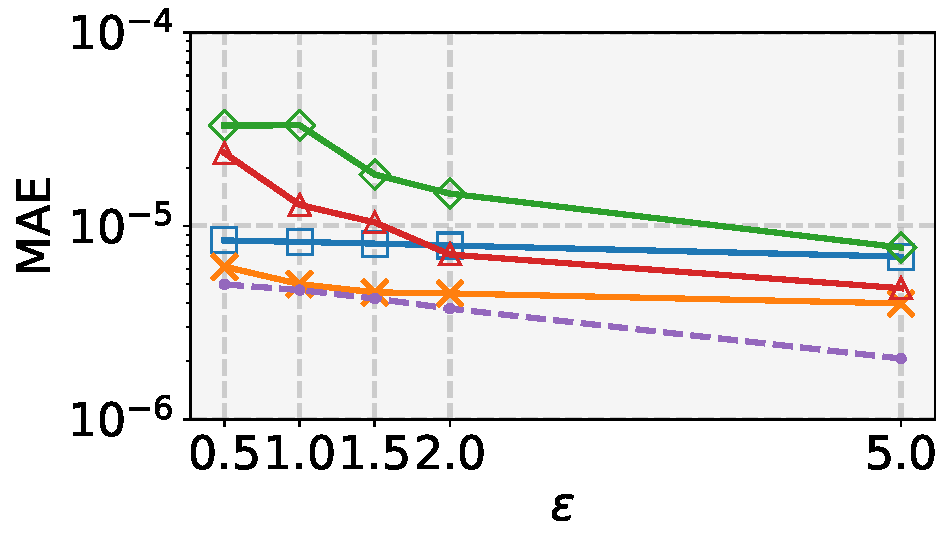
\includegraphics[width=.25\linewidth]{figs/w=20-tist-MAE.pdf}}
  \subfloat[Foursquare ($\epsilon=1$)]{%
    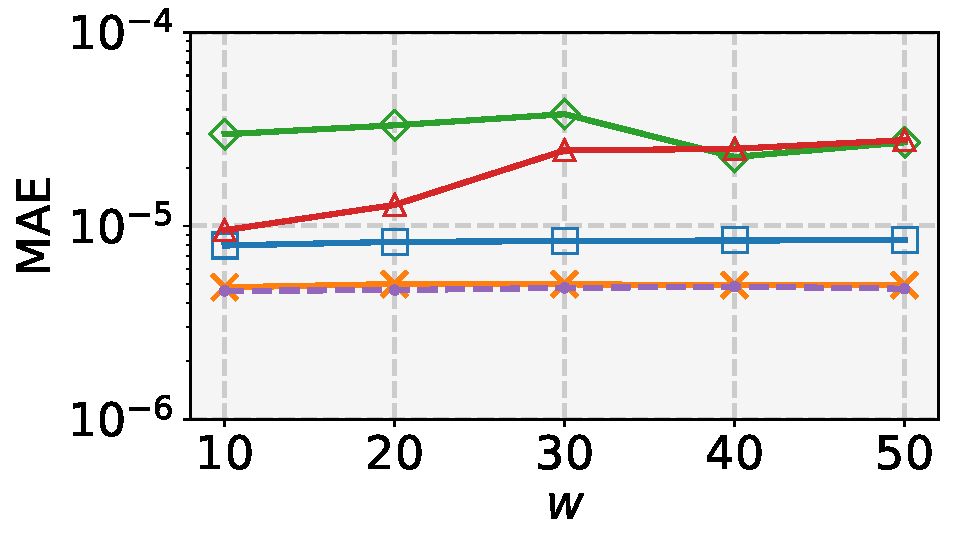
\includegraphics[width=.25\linewidth]{figs/e=1-tist-MAE.pdf}}
  \caption{Counting query evaluation with varying $\epsilon$ and $w$}
  \label{fig:histogram}
  \Description{The figure presents a 4x4 grid of line charts evaluating the performance of counting queries. 
The rows correspond to four datasets: Cosmetics, Taxi, Loan, and Foursquare. 
The columns represent different metrics and varying parameters: the first and second columns show Mean Relative Error (MRE) varying epsilon and window size w, respectively; the third and fourth columns show Mean Absolute Error (MAE) varying epsilon and w. 
Five methods are compared: LBU, LSP, LBD, LBA, and the proposed MTSP-LDP. 
In all 16 subplots, the Y-axis is on a logarithmic scale. 
Visually, the proposed MTSP-LDP method (represented by a purple dashed line) consistently stays at the bottom of all charts, indicating it achieves the lowest error by a significant margin (often orders of magnitude) compared to the four baseline methods across all datasets and parameter settings.}
\end{figure*}


In order to compare MTSP-LDP fairly with other baselines which are mainly
designed for frequency histogram estimation, we let $\hat\theta_{t,v}\triangleq
Q_t^c(v,1)/n_t$, and hence $\{\hat\theta_{t,v}\}_{v\in\Omega}$ is an estimate of
the frequency histogram of the stream at time $t$.
Then we evaluate the MAE and MRE of $\hat\theta_{v,t}$, averaged over time, and show
the results on the four datasets in \cref{fig:histogram}.

We observe that, for a fixed sliding window size $w$, as the privacy budget
$\epsilon$ increases from $0.5$ (i.e., high privacy protection) to $5$ (i.e., low
privacy protection), the estimation error for all algorithms decreases.
Similarly, for a fixed privacy budget $\epsilon$, as the window size $w$
increases from $10$ to $50$, the estimation error increases accordingly.
These results highlight a clear trade-off between privacy and data utility,
where larger privacy budgets or smaller window sizes generally lead to better
utility.

Notably, MTSP-LDP delivers consistently high accuracy across diverse datasets.
As discussed in \cref{sec:method}, this can be attributed to the fact that
existing algorithms do not fully leverage the temporal correlations in the data
stream when allocating privacy budgets.
Although the LBD and LBA methods conserve privacy budgets during periods of
minimal data change, their strategies focus solely on the current timestamp
without considering the data distribution across the entire time window.
This limitation is particularly critical in the $w$-event setting, where
capturing the overall data distribution is crucial for accurate estimates.
Besides, MTSP-LDP demonstrates a particularly significant advantage when the
privacy budget is small, as smaller budgets inherently introduce larger errors,
amplifying the weaknesses of other methods.
This makes MTSP-LDP highly effective in scenarios requiring strict privacy
guarantees.


\subsubsection{Evaluation for Range Queries}

\begin{figure*}[t]
  \centering
  
\includegraphics[width=.4\linewidth]{figs/legend_methods.pdf}

  \subfloat[Cosmetics ($w=20$)]{%
    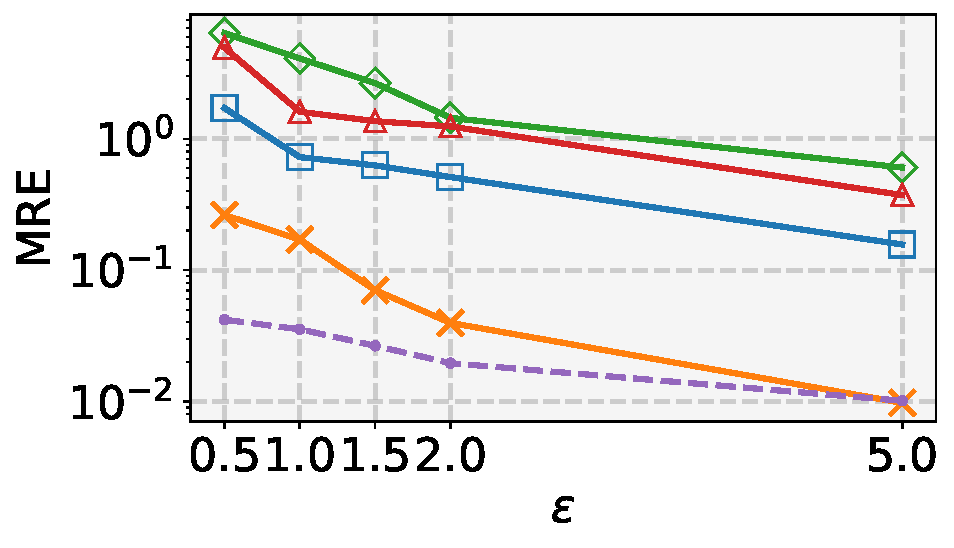
\includegraphics[width=.25\linewidth]{figs/query-w=20-category.pdf}}
  \subfloat[Cosmetics ($\epsilon=1$)]{%
    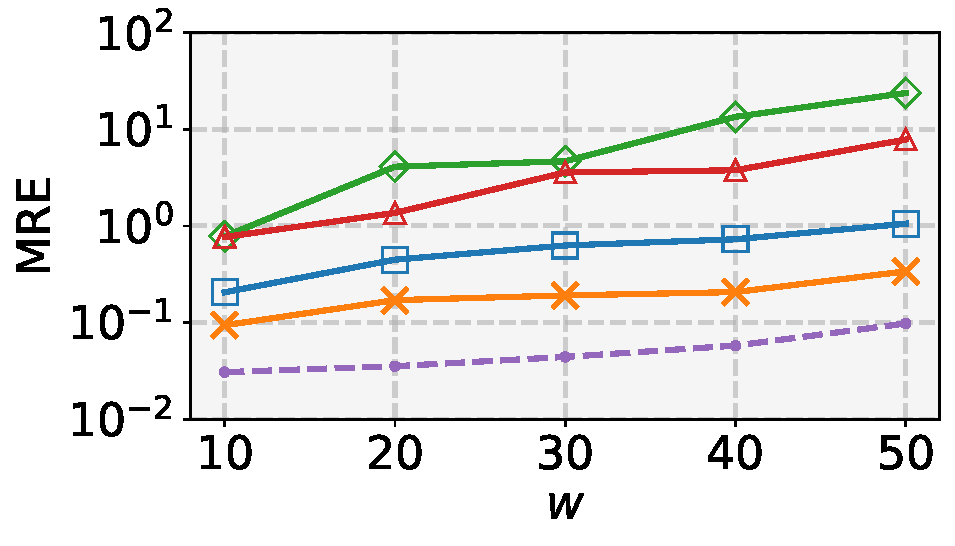
\includegraphics[width=.25\linewidth]{figs/query-e=1-category.pdf}}
  \subfloat[Cosmetics ($w=20$)]{%
    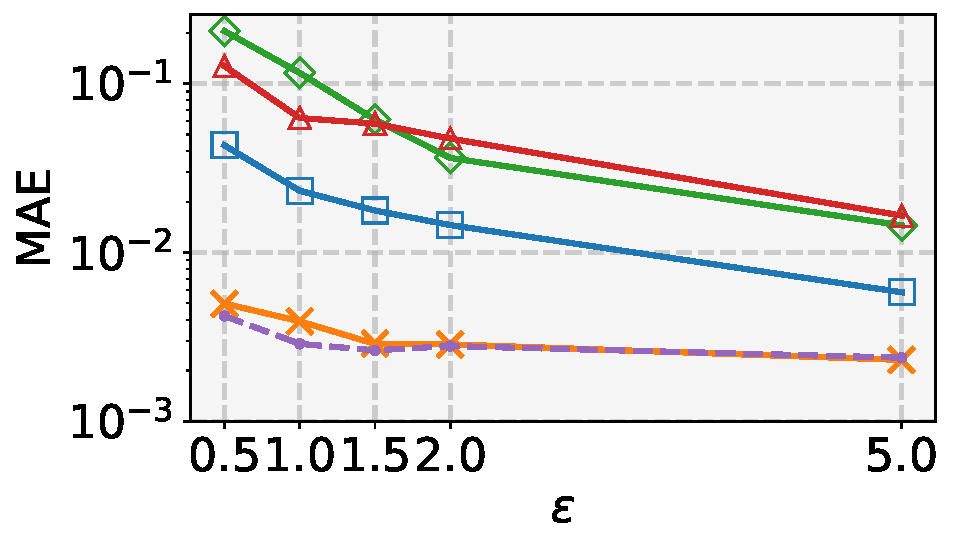
\includegraphics[width=.25\linewidth]{figs/query-w=20-category-MAE.pdf}}
  \subfloat[Cosmetics ($\epsilon=1$)]{%
    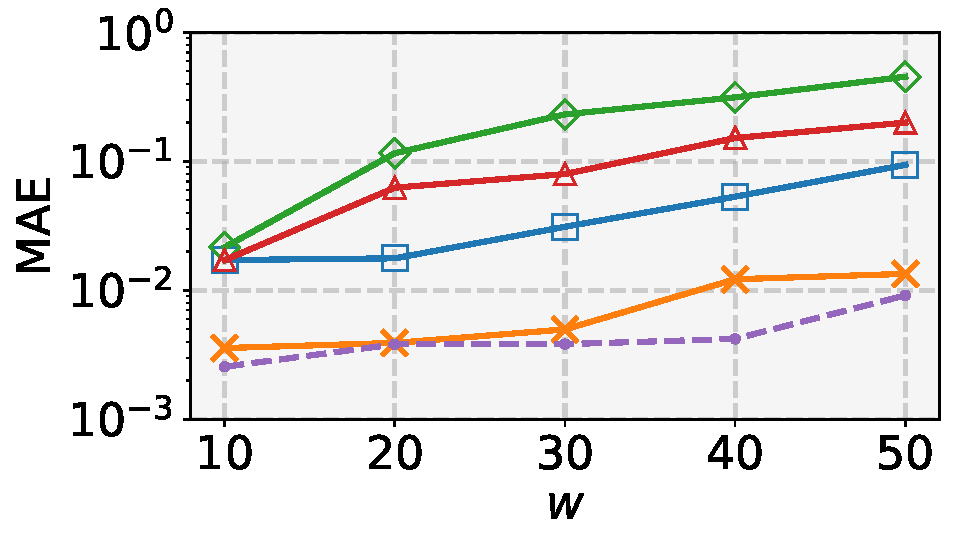
\includegraphics[width=.25\linewidth]{figs/query-e=1-category-MAE.pdf}}

  \subfloat[Taxi ($w=20$)]{%
    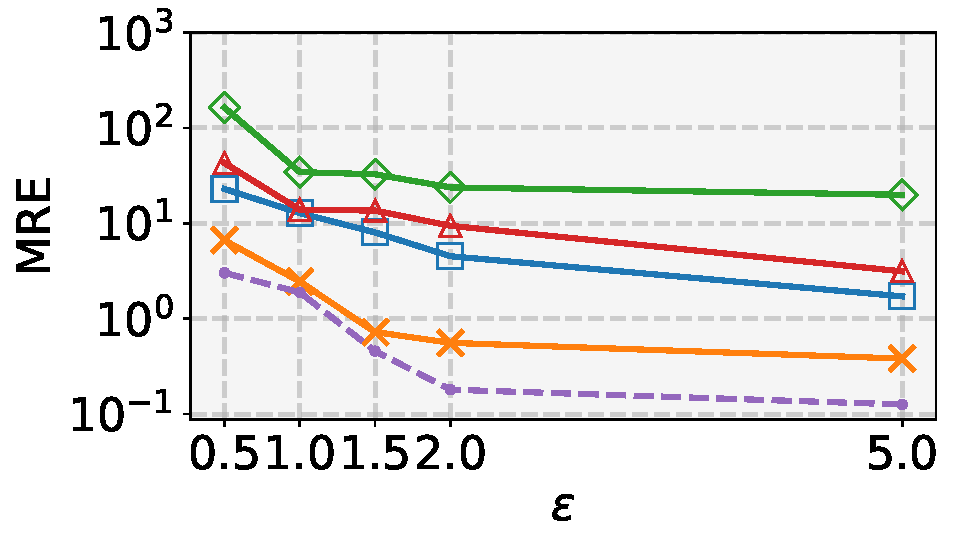
\includegraphics[width=.25\linewidth]{figs/query-w=20-taxi.pdf}}
  \subfloat[Taxi ($\epsilon=1$)]{%
    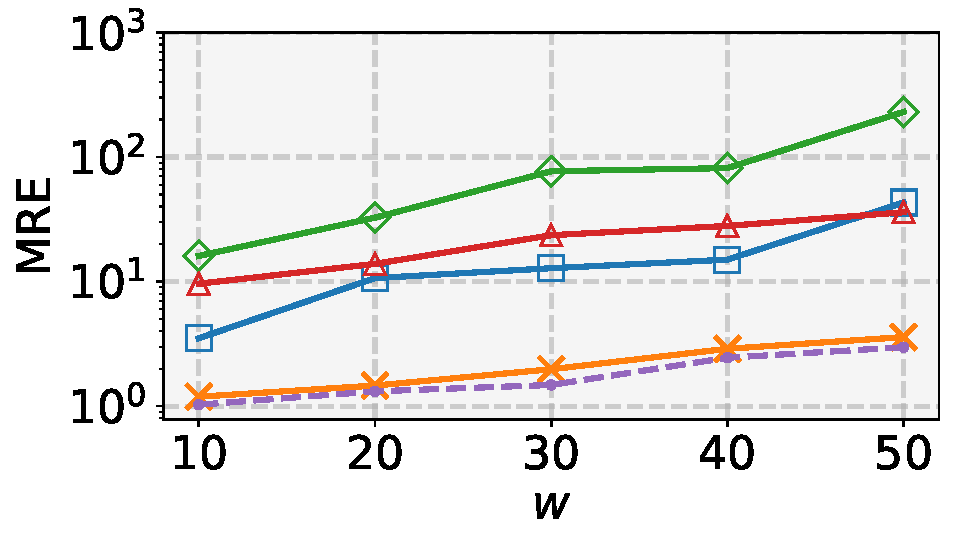
\includegraphics[width=.25\linewidth]{figs/query-e=1-taxi.pdf}}
  \subfloat[Taxi ($w=20$)]{%
    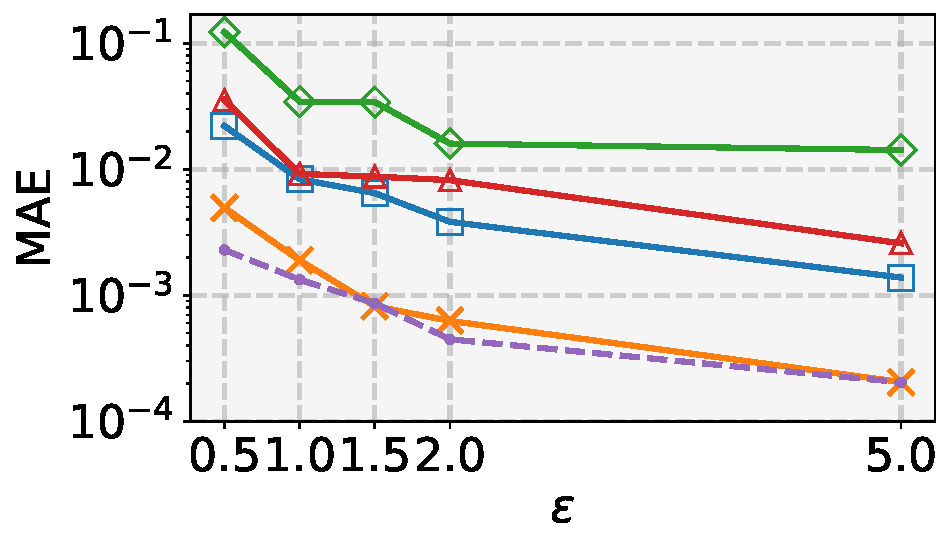
\includegraphics[width=.25\linewidth]{figs/query-w=20-taxi-MAE.pdf}}
  \subfloat[Taxi ($\epsilon=1$)]{%
    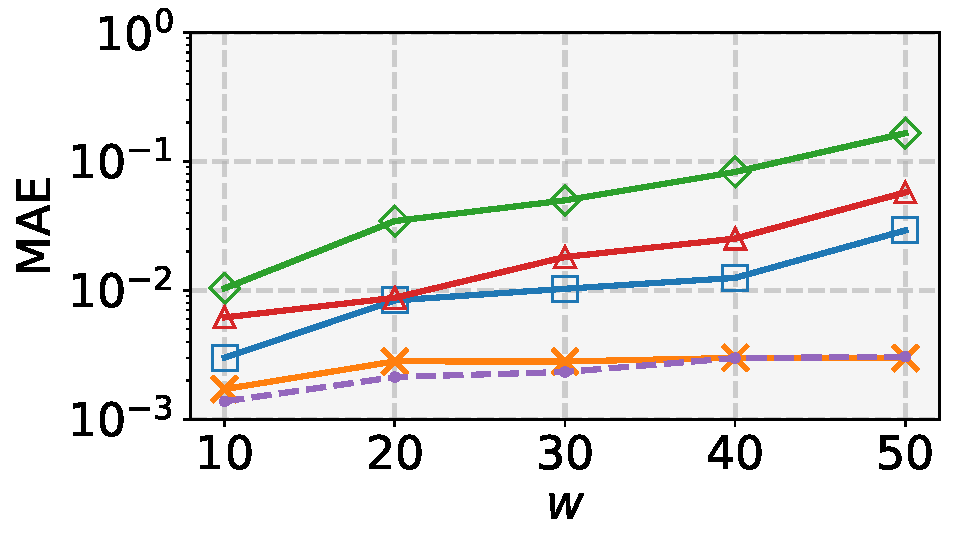
\includegraphics[width=.25\linewidth]{figs/query-e=1-taxi-MAE.pdf}}

  \subfloat[Loan ($w=20$)]{%
    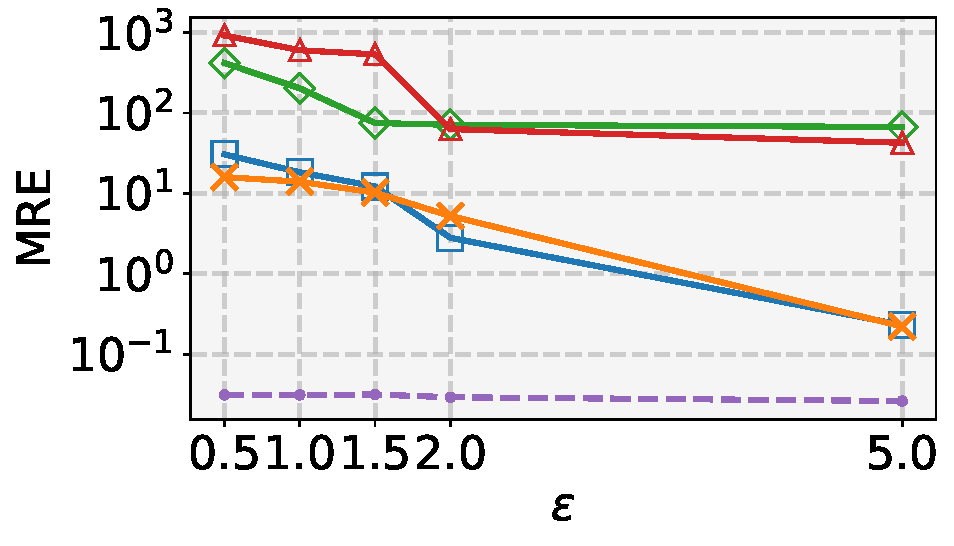
\includegraphics[width=.25\linewidth]{figs/query-w=20-loan.pdf}}
  \subfloat[Loan ($\epsilon=1$)]{%
    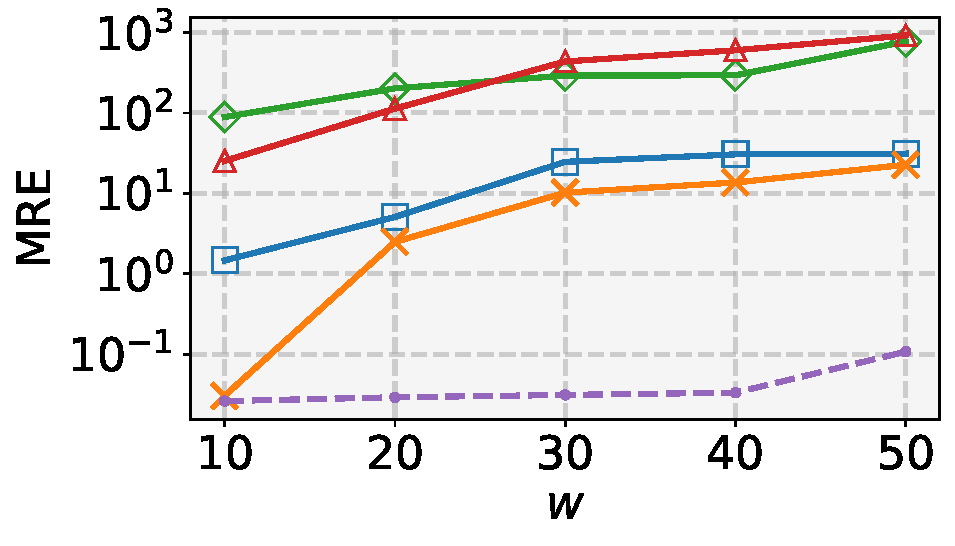
\includegraphics[width=.25\linewidth]{figs/query-e=1-loan.pdf}}
  \subfloat[Loan ($w=20$)]{%
    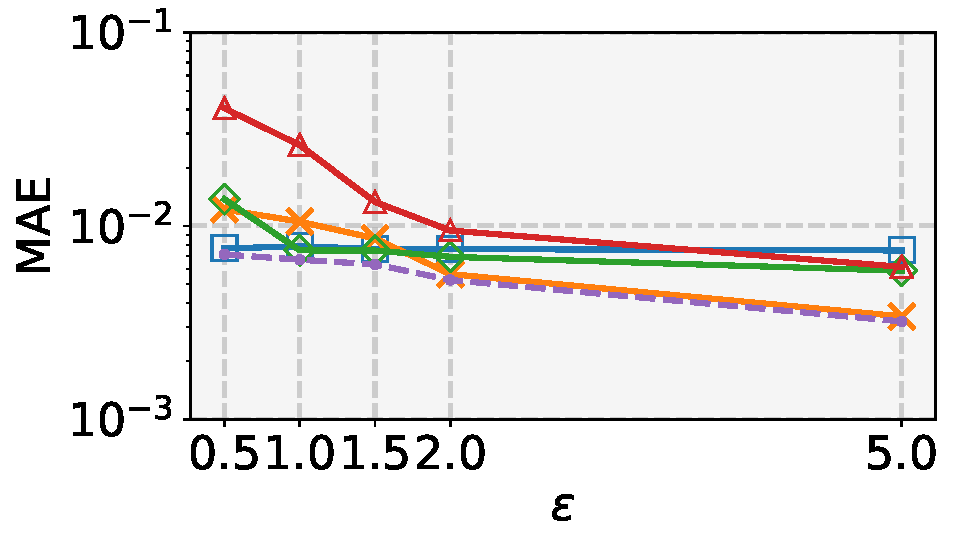
\includegraphics[width=.25\linewidth]{figs/query-w=20-loan-MAE.pdf}}
  \subfloat[Loan ($\epsilon=1$)]{%
    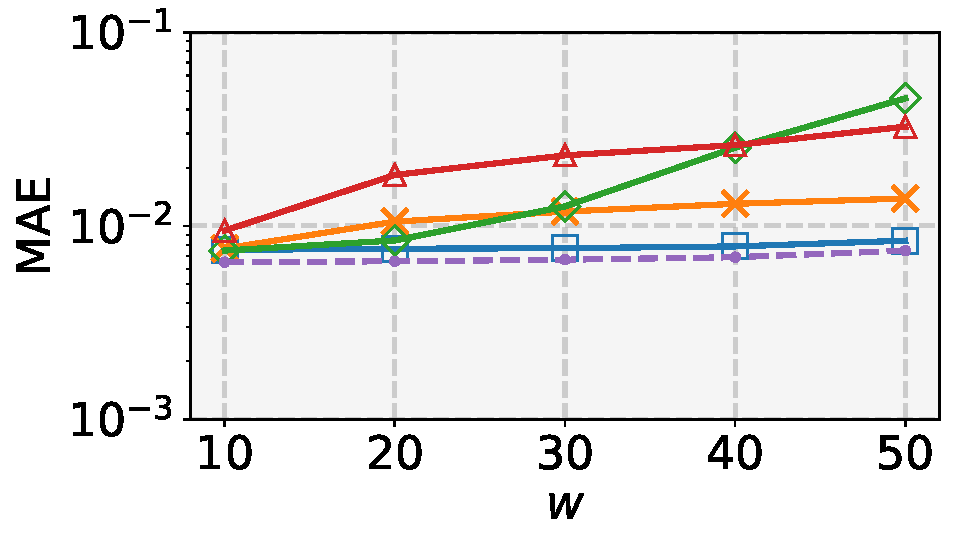
\includegraphics[width=.25\linewidth]{figs/query-e=1-loan-MAE.pdf}}

  \subfloat[Foursquare ($w=20$)]{%
    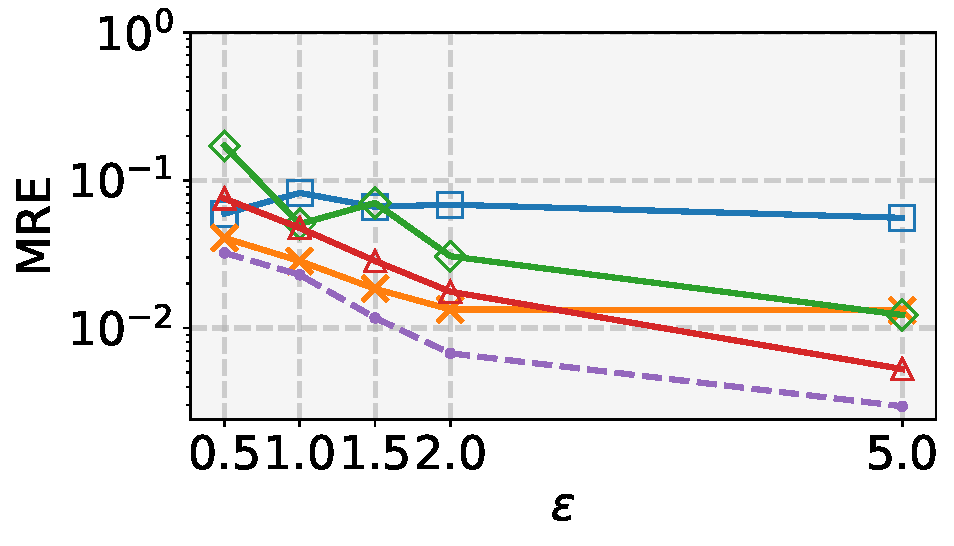
\includegraphics[width=.25\linewidth]{figs/query-w=20-tist.pdf}}
  \subfloat[Foursquare ($\epsilon=1$)]{%
    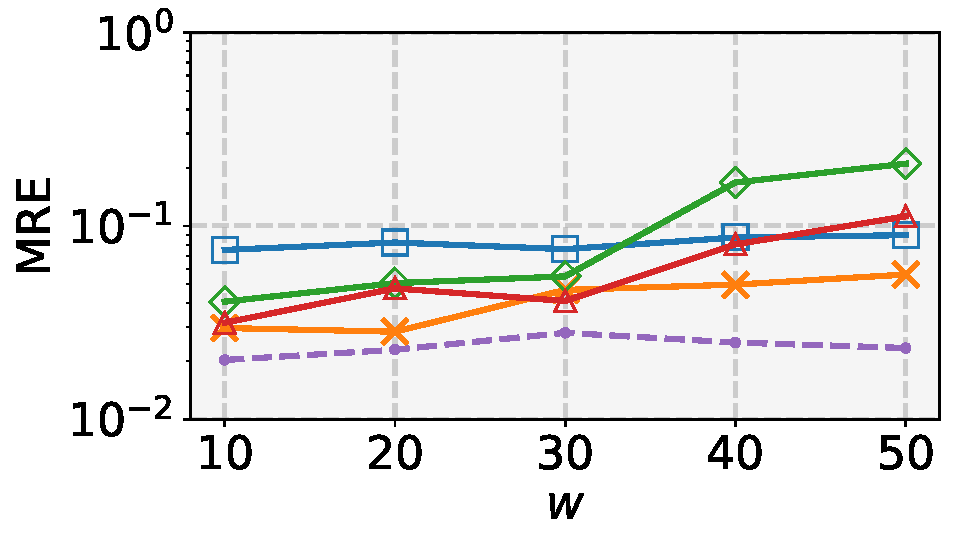
\includegraphics[width=.25\linewidth]{figs/query-e=1-tist.pdf}}
  \subfloat[Foursquare ($w=20$)]{%
    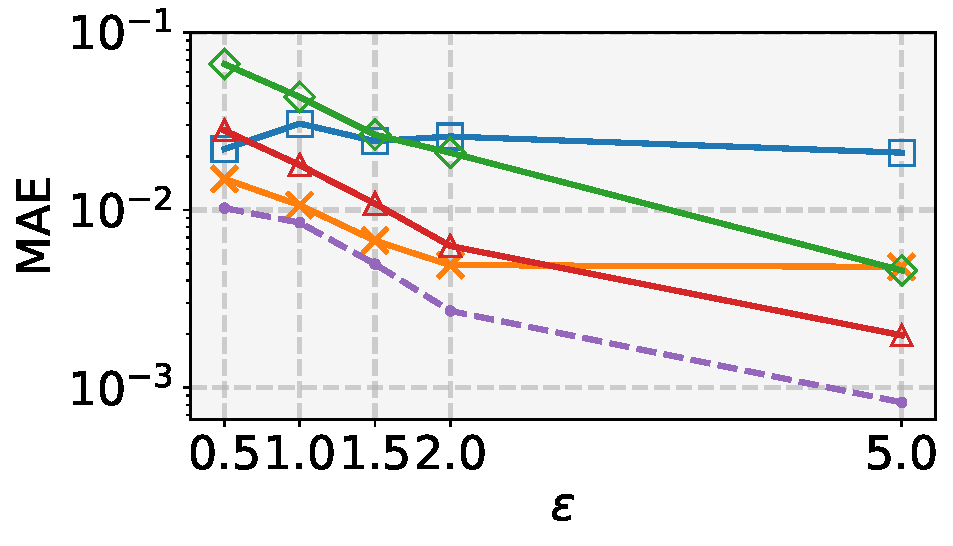
\includegraphics[width=.25\linewidth]{figs/query-w=20-tist-MAE.pdf}}
  \subfloat[Foursquare ($\epsilon=1$)]{%
    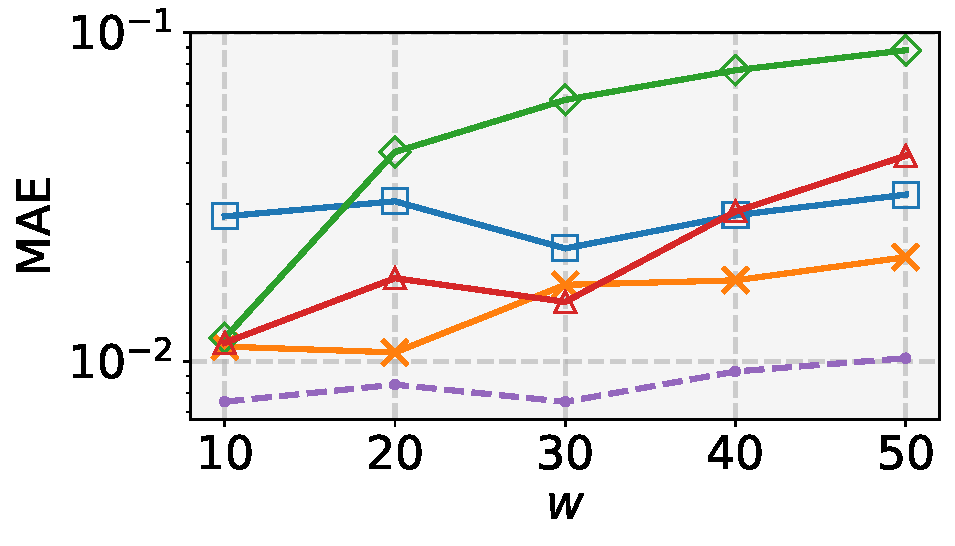
\includegraphics[width=.25\linewidth]{figs/query-e=1-tist-MAE.pdf}}
  \caption{Range query evaluation with varying $\epsilon$ and $w$}
  \label{fig:range_query}
  \Description{The figure presents a 4x4 grid of line charts evaluating the performance of range query. 
The rows correspond to four datasets: Cosmetics, Taxi, Loan, and Foursquare. 
The columns represent different metrics and varying parameters: the first and second columns show Mean Relative Error (MRE) varying epsilon and window size w, respectively; the third and fourth columns show Mean Absolute Error (MAE) varying epsilon and w. 
Five methods are compared: LBU, LSP, LBD, LBA, and the proposed MTSP-LDP. 
In all 16 subplots, the Y-axis is on a logarithmic scale. 
Visually, the proposed MTSP-LDP method (represented by a purple dashed line) consistently stays at the bottom of all charts, indicating it achieves the lowest error by a significant margin (often orders of magnitude) compared to the four baseline methods across all datasets and parameter settings.}
\end{figure*}


For baseline methods with frequency histogram estimates
$\{\hat{f}_{t,v}\}_{v\in\Omega}$, we can obtain the estimate of a frequency range query by
\[
  \hat{f}_{t,[v_1,v_2]}
  \triangleq \sum_{t'=t-\Delta+1}^t\sum_{v\in[v_1,v_2]} \hat{f}_{t',v}.
\]
For MTSP-LDP, the corresponding estimate is
\[
  \hat\theta_{t,[v_1,v_2]}
  \triangleq \frac{Q_t^r([v_1,v_2],\Delta)}{\sum_{t'=t-\Delta+1}^t n_{t'}}.
\]
We randomly generate $50$ range query tasks with varying value ranges
$[v_1,v_2]$ and time spans $\Delta$.
For each query, the MRE and MAE between the estimates and ground truths are
computed, and the average MRE and MAE across all queries are reported.
The results are shown in \cref{fig:range_query}.
Note that some query tasks span time ranges exceeding the predefined window
size, which means the total privacy budget used by these queries exceeds the set
budget for a single window.
However, this condition applies equally to all methods, ensuring a fair
comparison.

We observe that MTSP-LDP consistently achieves the lowest estimation errors
across all settings, with particularly pronounced improvements in MRE,
demonstrating superior accuracy under normalized error metrics.
This is because other approaches do not account for the complexity of performing
complex query tasks on streaming data and instead rely solely on publishing
frequency histograms.
While frequency histograms can be used to derive results for complex queries,
their cumulative error grows proportionally with the query range, leading to a
sharp decline in data utility.
In contrast, MTSP-LDP's data-adaptive hierarchical structure and cross-timestamp
processing enable more precise estimation for such queries, especially under
tight privacy budgets.


\subsubsection{Evaluation for Event Monitoring}

For event monitoring, we define a specific task where the goal is to detect the
change in the range query in the entire value domain $\Omega$ with threshold
$\vartheta$ equal to the median of $\Omega$ in each dataset.
The two functions in the range query are defined as follows.
\begin{align*}
  \alpha(\Omega,\Delta) &= Q_t^r(\Omega,\Delta)-Q_{t-w+1}^r(\Omega,\Delta)\\
  \beta(x,\vartheta) &= \indr{x>\vartheta}
\end{align*}
By analyzing the changes across consecutive windows, we ensure a consistent
comparison of each algorithm's ability to capture dynamic variations in the data
streams.
To better understand each method's performance, we vary the threshold
$\vartheta$, and obtain the ROC curve for each dataset, as illustrated in
\cref{fig:ROC_query}.

\begin{figure*}[t]
  \centering
  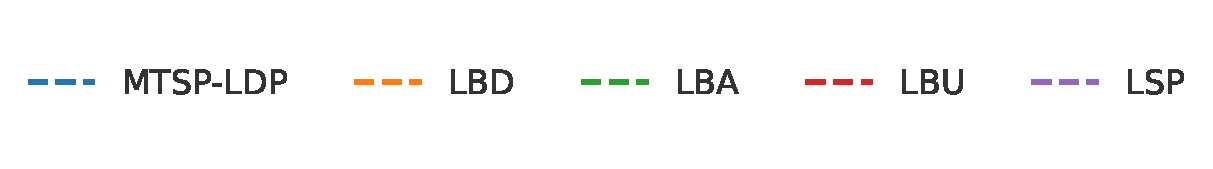
\includegraphics[width=.4\linewidth]{figs/legend_roc.pdf}\\[-2ex]
  \subfloat[Cosmetics]{%
    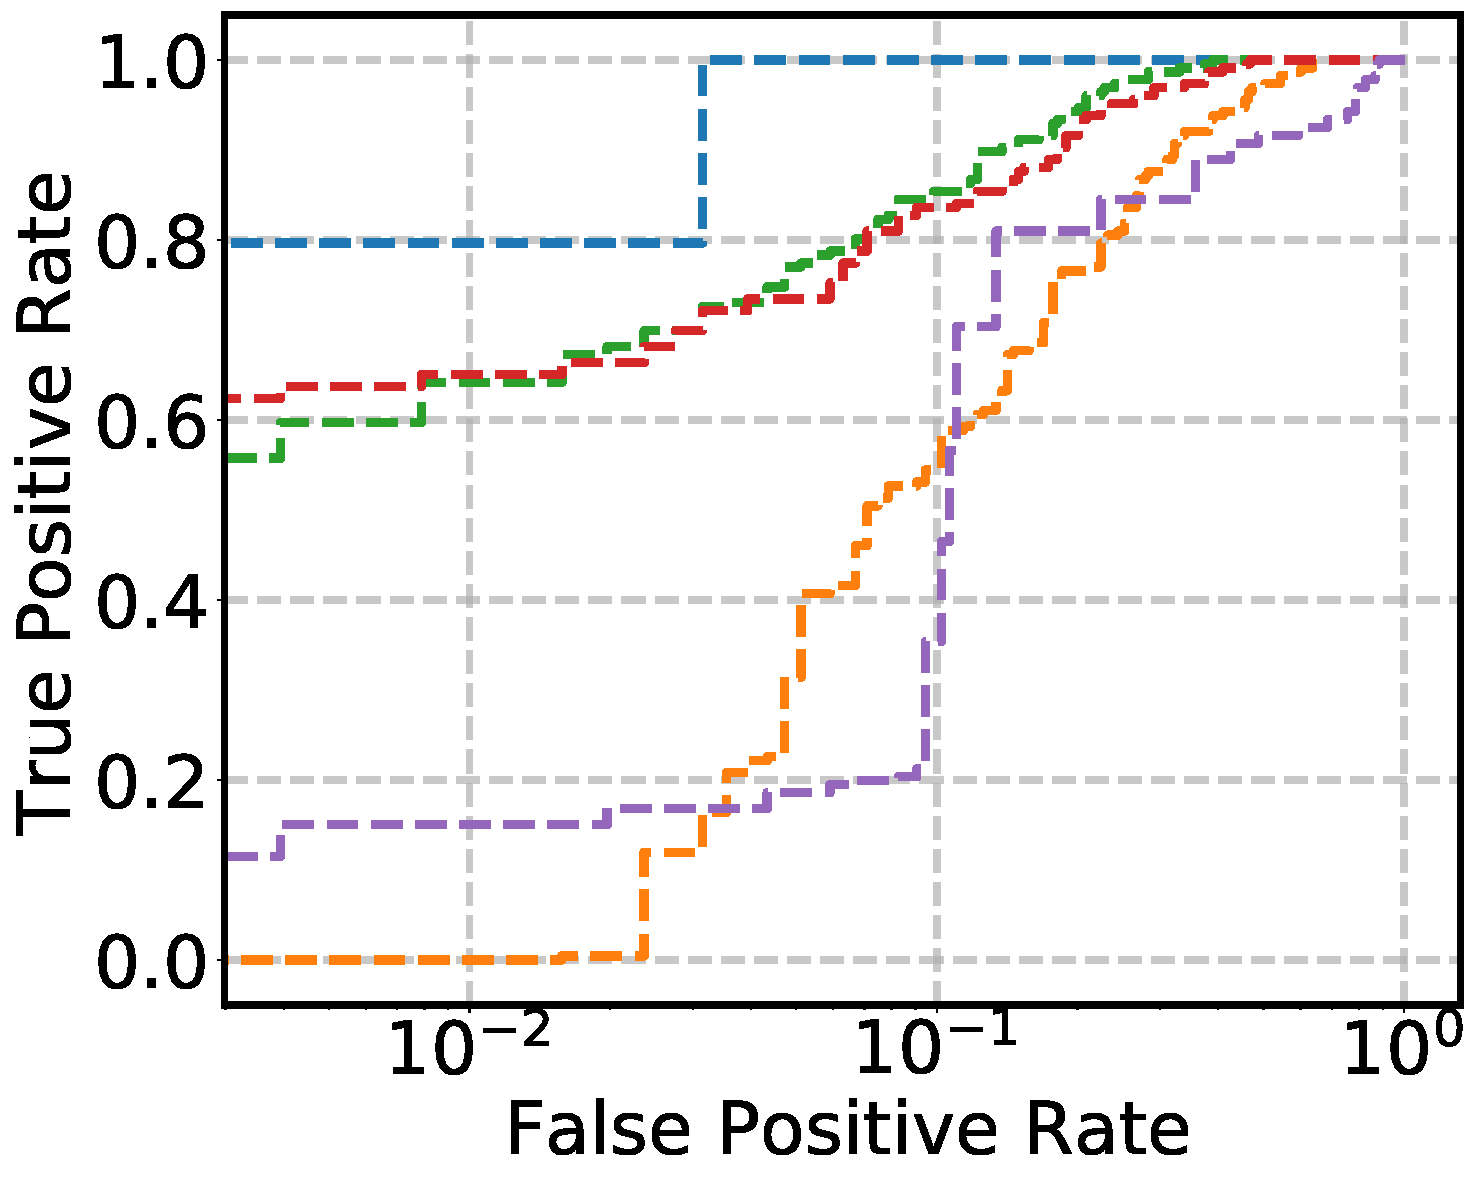
\includegraphics[width=.22\linewidth]{figs/ROC-category-w=20_2.pdf}}\quad
  \subfloat[Taxi]{%
    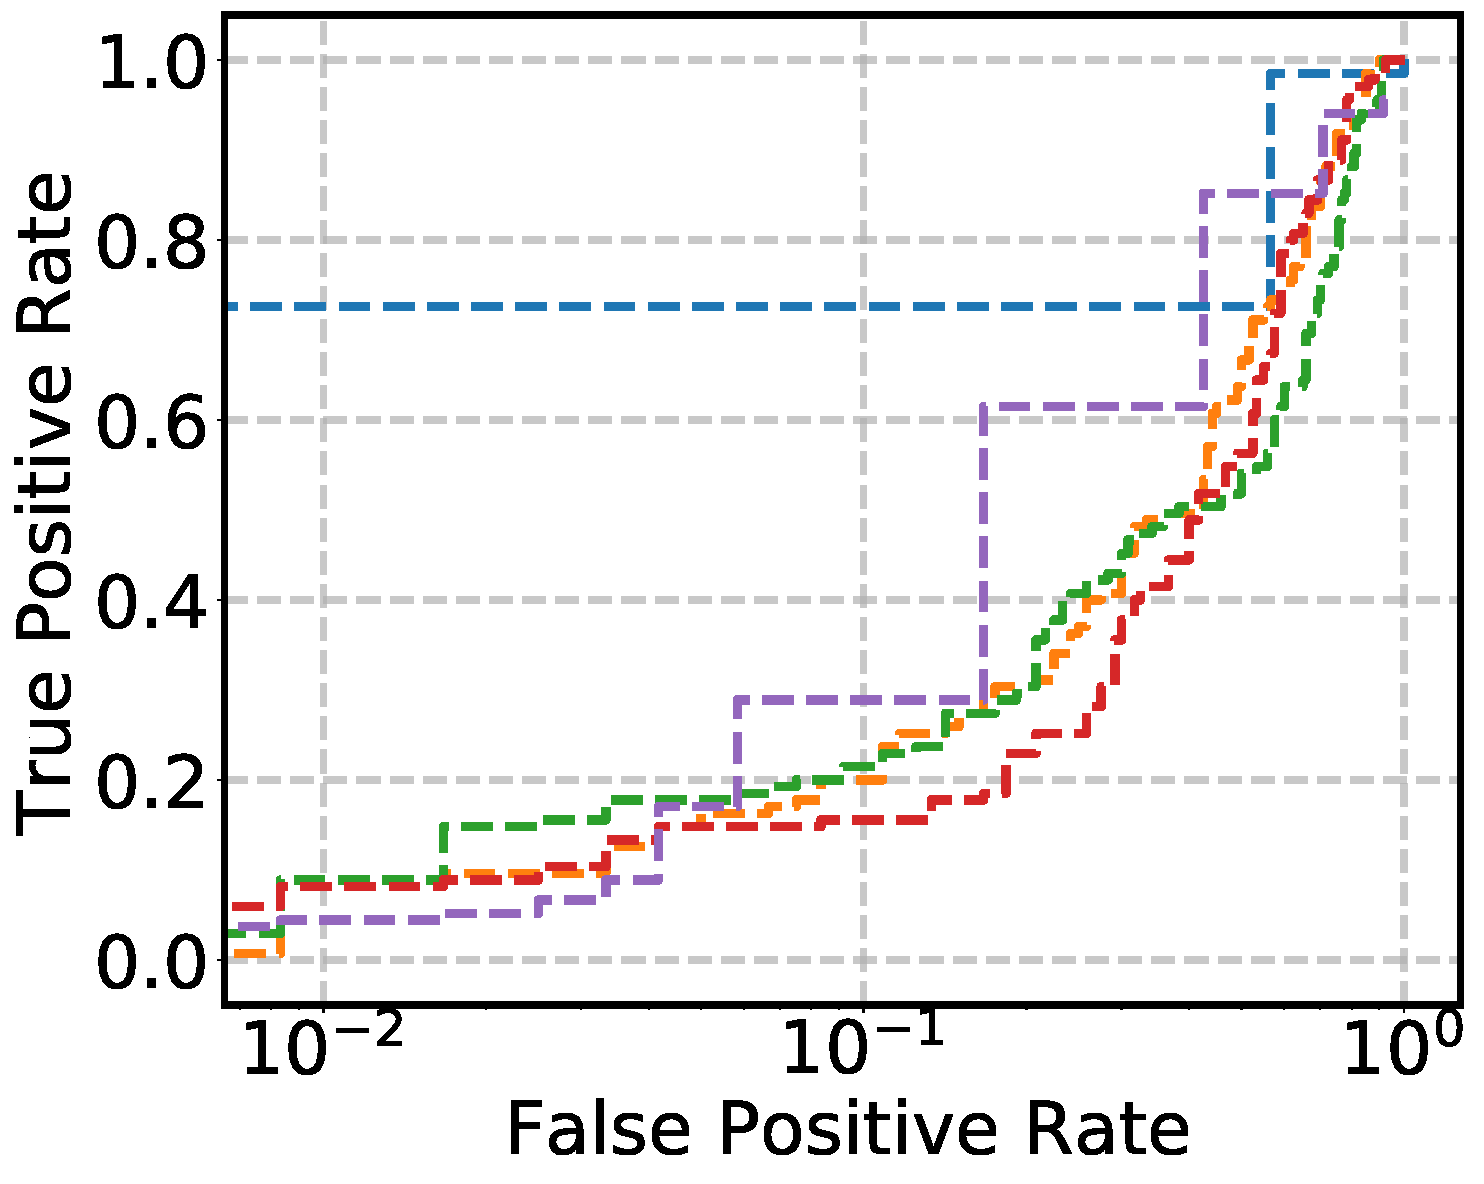
\includegraphics[width=.22\linewidth]{figs/ROC-taxi-w=20_2.pdf}}\quad
  \subfloat[Loan]{%
    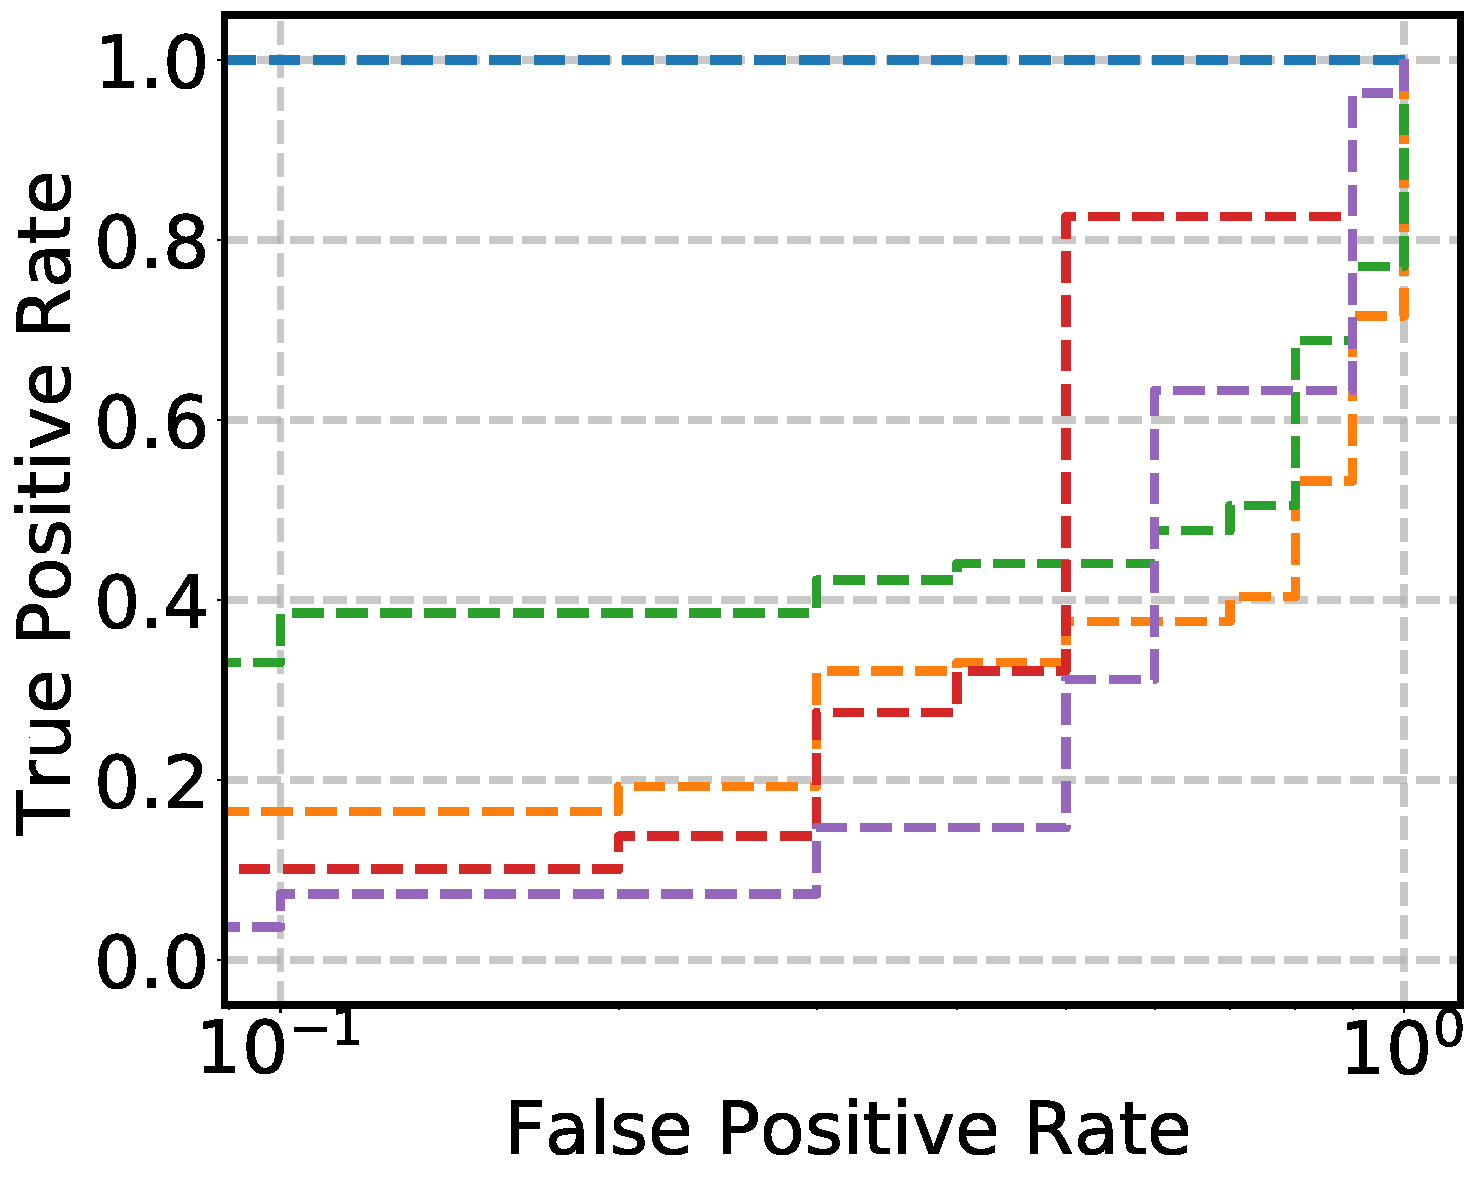
\includegraphics[width=.22\linewidth]{figs/ROC-loan-w=20_2.pdf}}\quad
  \subfloat[Foursquare]{%
    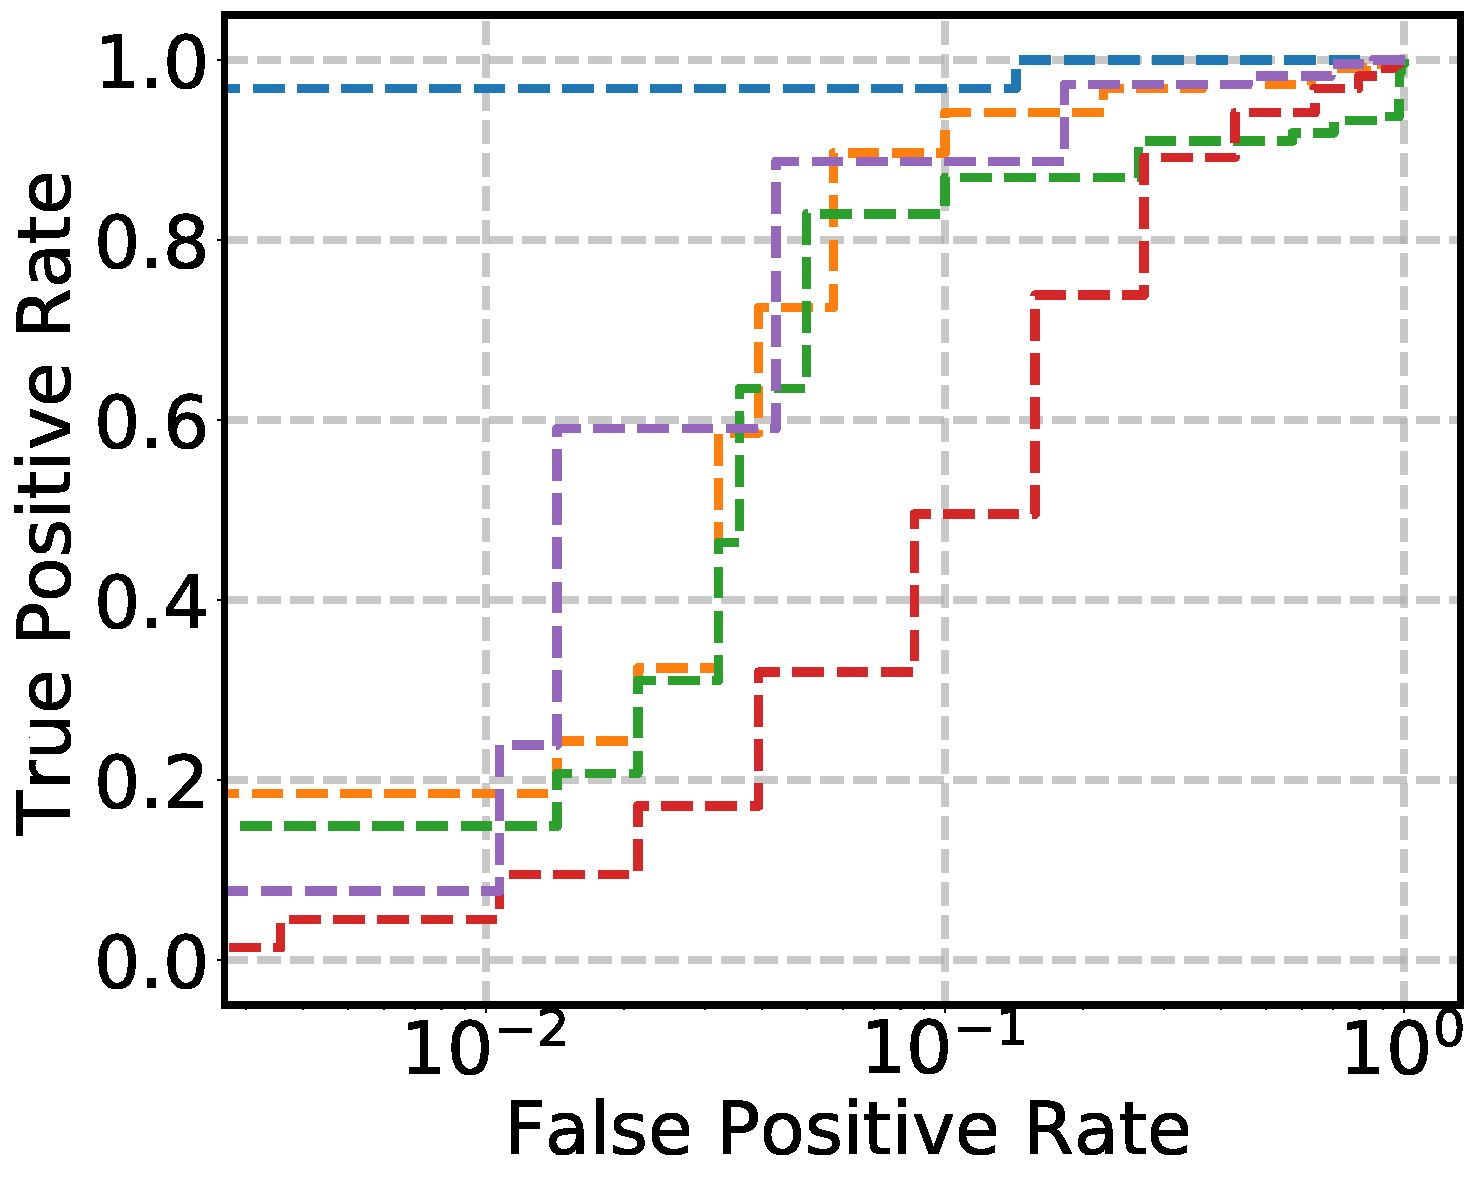
\includegraphics[width=.22\linewidth]{figs/roc_curve-tist-w=30.pdf}}
  \caption{ROC for event monitoring with $\epsilon=1$ and $w=20$}
  \label{fig:ROC_query}
  \Description{The figure displays four Receiver Operating Characteristic (ROC) curves corresponding to the Cosmetics, Taxi, Loan, and Foursquare datasets. 
The X-axis represents the False Positive Rate on a logarithmic scale, and the Y-axis represents the True Positive Rate. 
Five methods are compared: the proposed MTSP-LDP (blue dashed line) and four baselines (LBD, LBA, LBU, LSP). 
In all four subplots, the curve for MTSP-LDP rises most steeply and stays closest to the top-left corner, indicating it achieves the highest True Positive Rate while maintaining a low False Positive Rate. 
The baseline methods generally lag significantly behind, requiring much higher False Positive Rates to achieve comparable detection performance.}
\end{figure*}

We observe that MTSP-LDP consistently outperforms the other methods, attaining
near-perfect TPR across the full range of FPR.
This demonstrates the robustness and adaptability of MTSP-LDP to different data
distributions.
At low FPR levels (FPR$<0.1$), MTSP-LDP achieves significantly higher TPR
compared to other methods, highlighting its superior sensitivity under strict
false positive constraints.
In contrast, LBD and LBA exhibit limited performance, with slower TPR growth as
FPR increases.
While LSP shows relatively strong performance on the cosmetics dataset,
approaching MTSP-LDP in some regions, it still falls short of MTSP-LDP's
consistent accuracy across all datasets.

These results underscore the effectiveness of MTSP-LDP in addressing complex
query tasks under varying privacy constraints and data characteristics.
Its ability to achieve high accuracy across diverse datasets highlights its
suitability for real-world applications requiring stringent privacy guarantees
and robust performance.
